% =====================================================================================================
\section{Security Evaluation}\label{sec:security}
\subsection{Setup}
We measure what a keyless observer can reconstruct. For every frame we take the better of two pictures: the protected stream decoded as is, and a \emph{replacement attack} that substitutes fixed guesses for the encrypted values (absolute values for encrypted signs, the smallest value of the size category for encrypted amplitudes, zero DC differences) and re-encodes a valid JPEG. Leakage is the edge correlation~\eqref{eq:edge} of this picture with the original; we also report SSIM~\cite{ssim}. Sources are a synthetic corridor scene; \NumClips{} clips that we analyse but do not reproduce (two film trailers, two talking-head videos and a handheld phone video, identified by hash); \NumOpenClips{} openly licensed films of the Blender Foundation, the Sintel trailer and Tears of Steel (CC~BY~3.0)\footnote{\url{https://durian.blender.org}, \url{https://mango.blender.org}}; and the 24 images of the Kodak set\footnote{\url{http://r0k.us/graphics/kodak/}}. Video is resized to 320$\times$240 and sampled every 150 frames; frames without edges are excluded.

\textit{Format compliance.} The protected streams of \AllDecode{} six levels decode without error in \Decoders{}, at the original resolution, as Lemma~\ref{lem:format} requires.

\subsection{Outline leakage}\label{sec:leakage}
\begin{figure*}[t]
\centering
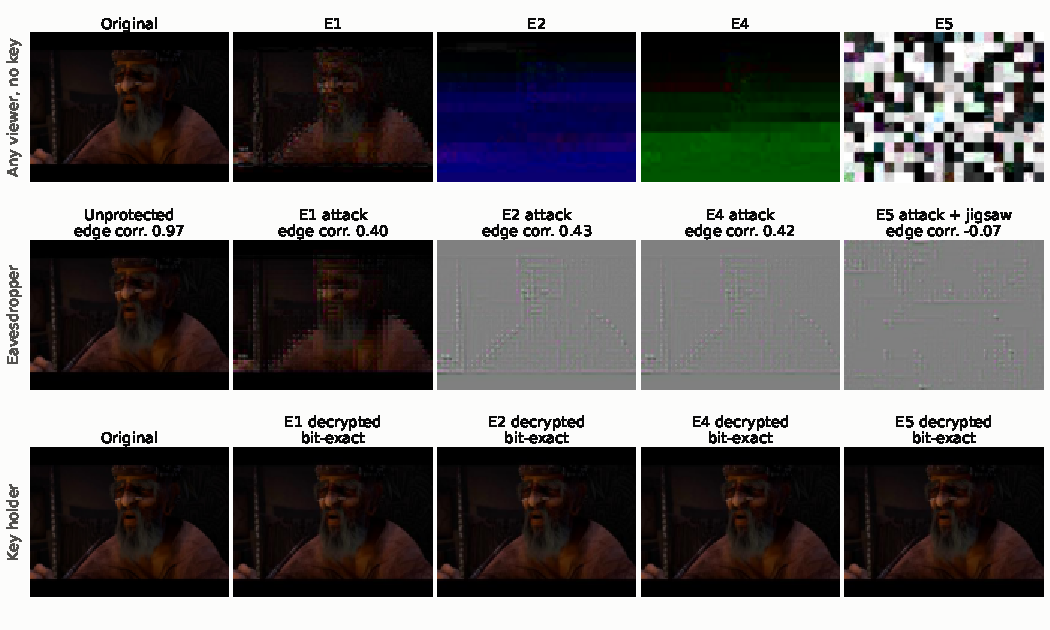
\includegraphics[width=0.66\textwidth]{figures/fig_visual_grid.pdf}
\caption{One frame of the Sintel trailer (\copyright{} Blender Foundation, CC~BY~3.0) per protection level. Top: what any viewer shows without the key. Middle: the eavesdropper's best reconstruction (replacement attack; for E5 followed by the jigsaw solver) with its edge correlation. Bottom: the key holder's output, bit-exact with the unprotected encoder.}
\label{fig:grid}
\end{figure*}
% generated by paper/make_assets.py from paper/data -- do not edit
\begin{table}[t]
\caption{Outline leakage: edge correlation between the original and the eavesdropper's best keyless reconstruction (decode or replacement attack; 0 = no outline), up to 60 frames per source; frames without edges are skipped. The first row is the fraction of payload bits encrypted. Jig.: share of neighbour pairs a greedy jigsaw solver restores under E5 (8 frames; Sintel 3); Oracle: edge correlation if every E5 block were put back in place, i.e.\ the outline E5 hides.}
\label{tab:leakage}
\centering\small\setlength{\tabcolsep}{4pt}
\resizebox{\columnwidth}{!}{%
\begin{tabular}{lrrrrrrrr}
\toprule
Source & E0 & E1 & E2 & E3 & E4 & E5 & Jig.\ (\%) & Oracle \\
\midrule
Enc.\ share & 0.00 & 0.11 & 0.13 & 0.26 & 0.29 & 0.31 & & \\
\midrule
Synthetic & 1.00 & 0.38 & 0.36 & 0.38 & 0.38 & 0.00 & 2.3 & 0.37 \\
Trailer A & 0.99 & 0.47 & 0.30 & 0.32 & 0.28 & 0.01 & 1.4 & 0.46 \\
Trailer B & 0.99 & 0.56 & 0.34 & 0.33 & 0.32 & 0.01 & 1.3 & 0.41 \\
Talk A & 0.99 & 0.51 & 0.45 & 0.44 & 0.44 & 0.01 & 1.4 & 0.45 \\
Talk B & 0.99 & 0.49 & 0.40 & 0.42 & 0.40 & 0.01 & 1.7 & 0.47 \\
Phone A & 0.99 & 0.45 & 0.35 & 0.34 & 0.33 & 0.00 & -- & -- \\
Sintel & 0.99 & 0.35 & 0.29 & 0.31 & 0.28 & -0.01 & 0.8 & 0.42 \\
Tears of Steel & 0.99 & 0.45 & 0.35 & 0.34 & 0.35 & -0.01 & 1.3 & 0.41 \\
Kodak & 0.99 & 0.39 & 0.33 & 0.34 & 0.31 & 0.00 & 1.3 & 0.32 \\
\bottomrule
\end{tabular}}
\end{table}

Fig.~\ref{fig:grid} and Table~\ref{tab:leakage} show the main effect. Under E1--E4 the eavesdropper sees a clear outline of the scene: edge correlation stays between \LeakEOneFourMin{} and \LeakEOneFourMax{} on the real sources, and encrypting amplitudes in addition to signs (E3, E4) does not reduce it, because the positions and size categories of the non-zero coefficients remain public (Lemma~\ref{lem:format}). The keyed macroblock permutation of E5 removes the outline (edge correlation between \LeakEFiveMin{} and \LeakEFiveMax). In terms of cost, E2 encrypts \CostEtwo\,\% of the payload bits, E4 \CostEfour\,\%, and E5 only slightly more, \CostEfive\,\%, yet only E5 moves leakage to zero.

% generated by paper/make_assets.py from paper/data -- do not edit
\begin{table}[t]
\caption{Edge correlation of the eavesdropper's best keyless picture with 95\,\% bootstrap intervals over the frames of each source (last column: frames).}
\label{tab:leakage_ci}
\centering\small\setlength{\tabcolsep}{3pt}
\resizebox{\columnwidth}{!}{%
\begin{tabular}{lccccr}
\toprule
Source & E1 & E2 & E4 & E5 & $n$ \\
\midrule
Synthetic & 0.38 {\scriptsize[0.37, 0.38]} & 0.36 {\scriptsize[0.36, 0.37]} & 0.38 {\scriptsize[0.37, 0.38]} & 0.00 {\scriptsize[-0.01, 0.00]} & 60 \\
Trailer A & 0.47 {\scriptsize[0.46, 0.49]} & 0.30 {\scriptsize[0.26, 0.34]} & 0.28 {\scriptsize[0.24, 0.33]} & 0.01 {\scriptsize[0.01, 0.02]} & 60 \\
Trailer B & 0.56 {\scriptsize[0.54, 0.58]} & 0.34 {\scriptsize[0.30, 0.38]} & 0.32 {\scriptsize[0.28, 0.36]} & 0.01 {\scriptsize[0.01, 0.02]} & 60 \\
Talk A & 0.51 {\scriptsize[0.49, 0.52]} & 0.45 {\scriptsize[0.42, 0.47]} & 0.44 {\scriptsize[0.42, 0.46]} & 0.01 {\scriptsize[0.00, 0.01]} & 60 \\
Talk B & 0.49 {\scriptsize[0.47, 0.51]} & 0.40 {\scriptsize[0.36, 0.43]} & 0.40 {\scriptsize[0.38, 0.43]} & 0.01 {\scriptsize[0.00, 0.01]} & 60 \\
Phone A & 0.45 {\scriptsize[0.44, 0.46]} & 0.35 {\scriptsize[0.32, 0.37]} & 0.33 {\scriptsize[0.31, 0.36]} & 0.00 {\scriptsize[0.00, 0.01]} & 60 \\
Sintel & 0.35 {\scriptsize[0.30, 0.41]} & 0.29 {\scriptsize[0.25, 0.33]} & 0.28 {\scriptsize[0.25, 0.31]} & -0.01 {\scriptsize[-0.01, 0.00]} & 25 \\
Tears of Steel & 0.45 {\scriptsize[0.42, 0.47]} & 0.35 {\scriptsize[0.30, 0.39]} & 0.35 {\scriptsize[0.30, 0.39]} & -0.01 {\scriptsize[-0.01, 0.00]} & 60 \\
Kodak & 0.39 {\scriptsize[0.36, 0.42]} & 0.33 {\scriptsize[0.27, 0.38]} & 0.31 {\scriptsize[0.27, 0.35]} & 0.00 {\scriptsize[0.00, 0.01]} & 24 \\
\bottomrule
\end{tabular}}
\end{table}

\begin{figure}[t]
\centering
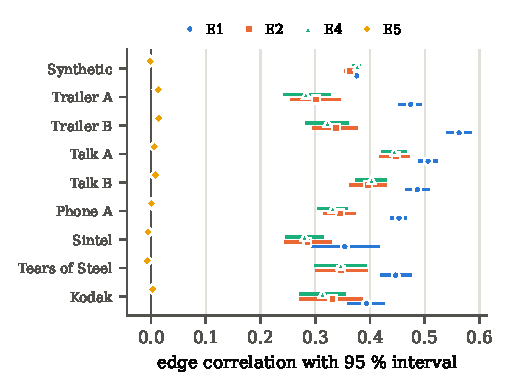
\includegraphics[width=\columnwidth]{figures/fig_leakage_ci.pdf}
\caption{Edge correlation of the eavesdropper's best keyless picture per source and level, with 95\,\% bootstrap intervals over up to \LeakFramesMax{} frames. E5's intervals lie at zero on every source; E1--E4 leak an outline everywhere.}
\label{fig:leakage_ci}
\end{figure}
\textit{Statistical confidence.} Table~\ref{tab:leakage_ci} and Fig.~\ref{fig:leakage_ci} give every leakage value with a 95\,\% percentile-bootstrap interval over the frames of its source. The intervals of E1--E4 are narrow and far from zero on all sources, so the outline leakage is not an effect of a few frames; the intervals of E5 contain zero or lie within a few hundredths of it.

\subsection{SVE-Bench: published schemes under the same attacks}\label{sec:bench}
% generated by paper/make_assets.py from paper/data -- do not edit
\begin{table*}[t]
\caption{SVE-Bench: format-compliant selective encryption schemes under the same attacks (175 frames of 9 sources, 320$\times$240, 768$\times$512). Values are edge correlations with the original (0: nothing leaks; plain JPEG sets the ceiling of each attack). A4 knows one frame in clear: it recovers the permutation and the keystream bits from that frame and applies them to the following frames. Published schemes re-implemented from their papers with our keystream.}
\label{tab:bench}
\centering\small
\resizebox{\textwidth}{!}{%
\begin{tabular}{lccrrrrrr}
\toprule
Scheme & Per-frame key & Auth. & Bytes (\%) & A1 decode & A2 replacement & A3 NZCA & A4 known plaintext & Max \\
\midrule
plain JPEG & -- & no & +0 & 0.94 & 0.94 & 0.79 & -- & \textbf{0.94} \\
\midrule
E1 & yes & yes & +1 & 0.47 & 0.41 & 0.79 & 0.47 & \textbf{0.79} \\
E2 & yes & yes & +1 & 0.14 & 0.41 & 0.79 & 0.14 & \textbf{0.79} \\
E3 & yes & yes & +1 & 0.14 & 0.40 & 0.79 & 0.15 & \textbf{0.79} \\
E4 & yes & yes & +1 & 0.15 & 0.40 & 0.79 & 0.14 & \textbf{0.79} \\
E5 (model) & yes & yes & +16 & 0.01 & 0.00 & 0.01 & 0.02 & \textbf{0.02} \\
E5 (hardware form) & yes & yes & +16 & 0.01 & 0.00 & 0.01 & 0.02 & \textbf{0.02} \\
\midrule
Van Droogenbroeck~\cite{vandroogenbroeck2002} & no & no & +0 & 0.47 & 0.40 & 0.79 & 0.94 & \textbf{0.94} \\
Kishore~\cite{kishore2015} & no & no & +0 & -0.00 & -0.00 & 0.00 & 0.78 & \textbf{0.78} \\
Auer~\cite{auer2013} & yes & no & +0 & 0.31 & 0.30 & 0.58 & 0.58 & \textbf{0.58} \\
Hirose, RI\,=\,1~\cite{hirose2024} & no & no & +15 & 0.00 & 0.01 & 0.01 & 0.90 & \textbf{0.90} \\
Hirose, RI\,=\,4~\cite{hirose2024} & no & no & +4 & 0.01 & 0.01 & 0.03 & 0.91 & \textbf{0.91} \\
\bottomrule
\end{tabular}}
\end{table*}

\begin{figure}[t]
\centering
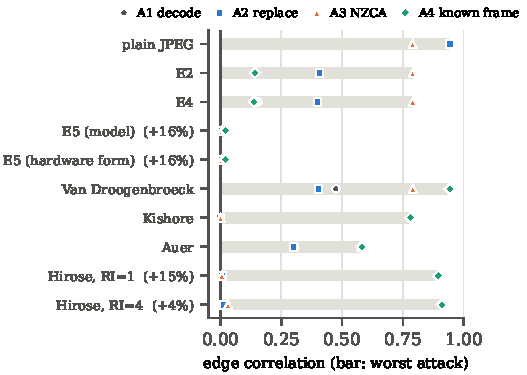
\includegraphics[width=\columnwidth]{figures/fig_bench.pdf}
\caption{SVE-Bench in one view: edge correlation of every scheme under each attack, pooled over \BenchSources{} sources; the bar ends at the worst attack. Byte cost over plain JPEG in brackets when above 2\,\%.}
\label{fig:bench}
\end{figure}
Leakage numbers from different papers are not comparable: each uses its own images, attack and metric. We therefore re-implemented four format-compliant schemes from their papers~\cite{vandroogenbroeck2002,kishore2015,auer2013,hirose2024}, with our keystream so that only the scheme differs, and scored them and ours under the same four attacks on \BenchFrames{} frames of \BenchSources{} sources (Table~\ref{tab:bench}, Fig.~\ref{fig:bench}):
\begin{itemize}
\item[A1] decoding the protected stream as is;
\item[A2] the replacement attack;
\item[A3] non-zero counting: a picture built from the number of non-zero coefficients per block, which no field encryption hides~\cite{hirose2024};
\item[A4] a known-plaintext attacker that knows one frame in clear, recovers from it the permutation and the keystream bits of that frame, and applies them to the following frames.
\end{itemize}
At its strongest attack every published scheme leaks between \BenchPubMin{} and \BenchPubMax. Those with fixed key material fall to the one known frame, among them Hirose et al.\ with a restart marker after every block (\BenchHiroseOneCross), although it costs about as many bytes as E5 ($+$\BenchHiroseOneBytes\,\%). E1--E4 sit at the non-zero-counting ceiling of plain JPEG (\BenchPlainNzca). E5, whose keystream and permutation change with every frame (Proposition~\ref{prop:perm}), stays at or below \BenchEfiveMax{} under every attack, in both its model and its hardware form; a test checks that the pictures an eavesdropper makes of the two forms are pixel-identical. The difference between E5 and Hirose et al.\ with one block per segment is not the mechanism, which is the same, but that our permutation is keyed per frame.

% generated by paper/make_assets.py from paper/data -- do not edit
\begin{table*}[t]
\caption{The metrics image-encryption papers report, for every scheme of Table~\ref{tab:bench} (no-key picture; same frames). PSNR and SSIM of the luma against the original; entropy of the luma histogram (8: flat); correlation of adjacent pixels; NPCR/UACI between the pictures under two keys one bit apart, and between two frames one pixel apart. They were designed for full-image ciphers: a format-compliant scheme keeps the stream decodable by design, so read them next to Table~\ref{tab:bench}.}
\label{tab:bench-metrics}
\centering\small
\resizebox{\textwidth}{!}{%
\begin{tabular}{lrrrccc}
\toprule
Scheme & PSNR (dB) & SSIM & Entropy & Corr. h / v / d & NPCR / UACI key (\%) & NPCR / UACI 1 px (\%) \\
\midrule
plain JPEG & 42.7 & 0.97 & 5.93 & 0.90 / 0.90 / 0.86 & -- / -- & 0.1 / 0.0 \\
\midrule
E1 & 24.9 & 0.59 & 6.03 & 0.87 / 0.86 / 0.80 & 70.4 / 4.7 & 32.4 / 1.9 \\
E2 & 11.0 & 0.29 & 5.09 & 0.85 / 0.87 / 0.82 & 86.8 / 46.1 & 32.2 / 11.3 \\
E3 & 11.1 & 0.28 & 5.10 & 0.84 / 0.88 / 0.81 & 87.3 / 48.5 & 32.7 / 11.5 \\
E4 & 10.2 & 0.28 & 4.97 & 0.82 / 0.86 / 0.79 & 86.6 / 48.2 & 32.4 / 11.9 \\
E5 (model) & 8.0 & 0.15 & 7.00 & 0.91 / 0.90 / 0.83 & 94.9 / 34.4 & 46.8 / 15.0 \\
E5 (hardware form) & 8.0 & 0.14 & 6.99 & 0.91 / 0.90 / 0.83 & 95.0 / 34.3 & 0.3 / 0.0 \\
\midrule
Van Droogenbroeck~\cite{vandroogenbroeck2002} & 24.5 & 0.57 & 6.05 & 0.86 / 0.85 / 0.79 & 71.4 / 5.3 & 33.1 / 2.1 \\
Kishore~\cite{kishore2015} & 7.4 & 0.18 & 6.05 & 0.89 / 0.88 / 0.84 & 88.7 / 40.0 & 14.6 / 1.2 \\
Auer~\cite{auer2013} & 16.9 & 0.40 & 6.24 & 0.63 / 0.61 / 0.49 & 84.6 / 21.7 & 75.9 / 17.7 \\
Hirose, RI\,=\,1~\cite{hirose2024} & 8.0 & 0.14 & 7.00 & 0.91 / 0.90 / 0.83 & 95.2 / 34.7 & 46.7 / 14.9 \\
Hirose, RI\,=\,4~\cite{hirose2024} & 7.6 & 0.18 & 6.93 & 0.96 / 0.92 / 0.89 & 94.1 / 37.1 & 45.7 / 16.3 \\
\bottomrule
\end{tabular}}
\end{table*}

\textit{The metrics of image-encryption papers.} Table~\ref{tab:bench-metrics} gives, for every scheme, the metrics that image-encryption papers report. They rank the schemes differently from Table~\ref{tab:bench}: a scheme that scrambles symbols without hiding positions can score well on PSNR, entropy and NPCR while leaking its outline, because these metrics measure how noisy the picture looks, not what an attacker can extract from it.

\subsection{Jigsaw solvers and a chosen-plaintext attack}
\begin{figure}[t]
\centering
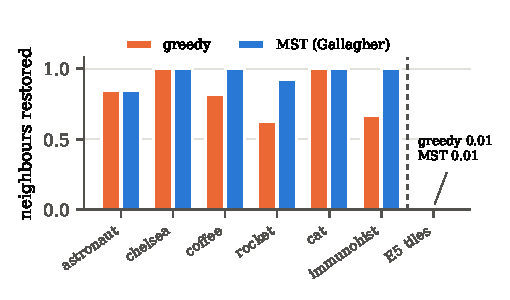
\includegraphics[width=\columnwidth]{figures/fig_jigsaw.pdf}
\caption{Neighbour pairs restored by the greedy and the minimum-spanning-tree solver on shuffled \emph{unencrypted} tiles of standard test photos (left) and on E5 tiles averaged over all sources (right).}
\label{fig:jigsaw}
\end{figure}
A permutation of blocks invites a puzzle solver. Our greedy region-growing solver in the style of~\cite{pomeranz2011} restores most neighbour relations on unencrypted shuffled tiles. On E5 replacement-attack tiles it places at most \JigsawNeighboursMax\,\% of neighbour pairs correctly, and the solved picture has no outline (Table~\ref{tab:leakage}). The structure is not destroyed, only hidden: an oracle that knew the permutation would recover edge correlations of \JigsawOracleMin--\JigsawOracleMax. A minimum-spanning-tree solver with Mahalanobis gradient compatibility~\cite{gallagher2012}, which restores at least \GateMstMin{} of the neighbours on unencrypted tiles of \GatePhotos{} photos (greedy: \GateGreedyMin), is also at chance on E5 (at most \MstNbMax\,\% on \MstSources{} sources, Fig.~\ref{fig:jigsaw}). The solvers fail because E5 also encrypts signs and amplitudes, so the borders of neighbouring tiles no longer match.

A chosen-plaintext attack~\cite{li2025shuffle} fails too: the attacker films a designed pattern whose per-block non-zero counts reveal the permutation. The permutation comes from the frame nonce, so on all \CpaSources{} sources one frame's exact permutation places at most \CpaPlacedEfive\,\% of the next frame's \CpaTiles{} tiles (chance) and leaves edge correlation $\le$\CpaEdgeEfive, where a key-only shuffle would give \CpaEdgeKeyMin--\CpaEdgeKeyMax.

\subsection{Sign-bit recovery by optimization}
% generated by paper/make_assets.py from paper/data -- do not edit
\begin{table}[t]
\caption{Sign-bit recovery attack of Lin et al.~\cite{lin2024} (LP relaxation, luma, 29 frames of 9 source sets). Top: their own setting on plain JPEG, where only the first $U$ AC signs per block are unknown (check of our implementation). Bottom: our levels, attacked from the ciphertext alone. Signs: share of unknown AC signs recovered, weighted by magnitude (chance 50\,\%). Edge: edge correlation with the original; last column: the replacement attack for comparison.}
\label{tab:signrec}
\centering\small
\resizebox{\columnwidth}{!}{%
\begin{tabular}{lrrrrr}
\toprule
Setting & Frames & Signs & SSIM & Edge & Repl.\ edge \\
\midrule
Lin et al.'s setting, $U{=}3$ & 29 & 93\,\% & 0.92 & 0.96 & -- \\
Lin et al.'s setting, $U{=}6$ & 29 & 88\,\% & 0.87 & 0.92 & -- \\
\midrule
E1 & 29 & 59\,\% & 0.45 & 0.41 & 0.33 \\
E2 & 29 & 49\,\% & 0.20 & 0.35 & 0.32 \\
E3 & 29 & -- & 0.21 & 0.36 & 0.31 \\
E4 & 29 & -- & 0.16 & 0.30 & 0.31 \\
\bottomrule
\end{tabular}}
\end{table}

The linear program of Lin et al.~\cite{lin2024} treats the unknown signs as relaxed variables and minimizes the total variation of the picture subject to the known magnitudes and the pixel range. In their setting, where only the first three or six AC signs of a block are unknown, it recovers \SrLinSignsMin--\SrLinSignsMax\,\% of the signs. On our levels it recovers \SrEoneSigns\,\% of E1's signs (\SrEoneSignsMin--\SrEoneSignsMax\,\% per frame), where every AC sign is hidden, and \SrEtwoSigns\,\% of E2's (chance 50\,\%) on \SrFrames{} frames of \SrSources{} source sets. It still sharpens E1's keyless picture (edge \SrEoneEdge{} against \SrEoneReplEdge{} for the replacement attack) and E2's and E3's by a few hundredths (Table~\ref{tab:signrec}): E1--E4 leak outlines however the hidden values are guessed.

\subsection{Learned attackers}
% generated by paper/make_assets.py from paper/data -- do not edit
\begin{table}[t]
\caption{U-Net reconstruction, SSIM / edge corr.\ on unseen test clips. P1: Trailer A$\rightarrow$B, P2: Talk A$\rightarrow$B, P3: Sintel$\rightarrow$Tears of Steel, P4: four sources$\rightarrow$three others. Repl.: replacement attack, P4 test set. Last row: the median training frame, scored without looking at the stream.}
\label{tab:learned}
\centering\small\setlength{\tabcolsep}{3pt}
\resizebox{\columnwidth}{!}{%
\begin{tabular}{llcccc}
\toprule
Mode & Repl. & P1 & P2 & P3 & P4 \\
\midrule
E1 & 0.57 / 0.40 & 0.72 / 0.53 & 0.70 / 0.66 & 0.55 / 0.41 & 0.79 / 0.69 \\
E2 & 0.21 / 0.39 & 0.42 / 0.33 & 0.27 / 0.34 & 0.14 / 0.31 & 0.37 / 0.43 \\
E4 & 0.22 / 0.38 & 0.43 / 0.34 & 0.28 / 0.32 & 0.13 / 0.30 & 0.36 / 0.37 \\
E5 & 0.18 / 0.01 & 0.34 / -0.02 & 0.26 / 0.02 & 0.22 / 0.00 & 0.34 / 0.03 \\
\midrule
No key, no stream & -- & -- & -- & 0.21 / 0.04 & 0.25 / -0.00 \\
\bottomrule
\end{tabular}}
\end{table}

% generated by paper/make_assets.py from paper/data -- do not edit
\begin{table}[t]
\caption{Learned attackers with controls, SSIM/edge correlation on unseen test sources. R: replacement attack; N: U-Net. P3: Sintel$\rightarrow$Tears of Steel; P4: four sources$\rightarrow$three others; P5: public corpus with an adversarial loss$\rightarrow$the Sintel trailer and the private clips. Controls use no ciphertext: the median training frame, recoloured with the frame statistics the E5 stream reveals or with the true ones.}
\label{tab:learned_ext}
\centering\small\setlength{\tabcolsep}{2.5pt}
\resizebox{\columnwidth}{!}{%
\begin{tabular}{lcccccc}
\toprule
 & \multicolumn{2}{c}{P3} & \multicolumn{2}{c}{P4} & \multicolumn{2}{c}{P5} \\
Mode & R & N & R & N & R & N \\
\midrule
E1 & 0.45/0.36 & 0.55/0.41 & 0.57/0.40 & 0.79/0.69 & 0.61/0.47 & 0.83/0.74 \\
E2 & 0.18/0.36 & 0.14/0.31 & 0.21/0.39 & 0.37/0.43 & 0.20/0.41 & 0.30/0.40 \\
E4 & 0.19/0.35 & 0.13/0.30 & 0.22/0.38 & 0.36/0.37 & 0.21/0.40 & 0.31/0.41 \\
E5 & 0.14/0.00 & 0.22/0.00 & 0.18/0.01 & 0.34/0.03 & 0.17/0.01 & 0.26/-0.01 \\
\midrule
No stream (median frame) &  & 0.21/0.04 &  & 0.25/0.00 &  & 0.28/0.06 \\
+ stats the stream reveals &  & 0.22/0.04 &  & 0.26/0.00 &  & 0.26/0.06 \\
+ true frame stats (oracle) &  & 0.23/0.04 &  & 0.36/0.04 &  & 0.36/0.08 \\
\bottomrule
\end{tabular}}
\end{table}

\begin{figure*}[t]
\centering
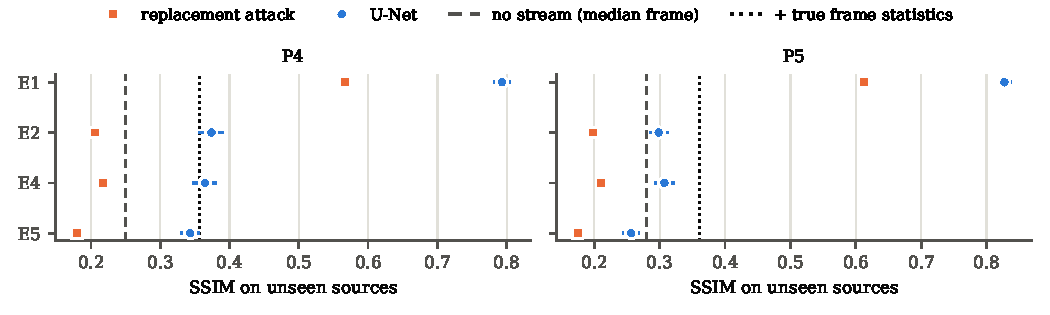
\includegraphics[width=0.85\textwidth]{figures/fig_learned.pdf}
\caption{SSIM of the learned attackers (U-Net, with 95\,\% interval) and of the replacement attack on unseen sources, per level. Dashed: the median training frame, which uses no ciphertext; dotted: the same frame recoloured with each test frame's true colour statistics. P4: four sources to three others; P5: trained on public films with an adversarial loss, tested on six other sources.}
\label{fig:learned}
\end{figure*}
We trained a U-Net~\cite{unet} to map the two keyless pictures (decoded and replacement attack) to the original and always tested it on clips it had not seen (Table~\ref{tab:learned}). P1 and P2 train on \LearnTrain{} frames of one clip, P3 uses only the open films, and P4 trains a wider network for \LearnBigEpochs{} epochs on \LearnBigTrain{} frames of \LearnBigTrainSrc{} sources and tests on \LearnBigTest{} frames of \LearnBigTestSrc{} others. The network defeats sign-only encryption: under E1 it reaches an edge correlation of \LearnEoneEdge{} and SSIM \LearnEoneSsim{} (replacement attack: \ReplEoneEdge{}), so E1 is no protection against a trained attacker. Under E2 and E4 it adds little to the outline that replacement already reveals (edge correlation \LearnEtwoFourEdgeMin--\LearnEtwoFourEdge{} against \ReplEtwoFourEdge) but raises SSIM to about \LearnEtwoFourSsimBig{} by learning brightness and colour.

\textit{Controls for frame-level statistics.} Table~\ref{tab:learned_ext} and Fig.~\ref{fig:learned} compare each learned attacker with three pictures that use no ciphertext: the median training frame, the same frame recoloured with the mean and spread of colour that the E5 stream itself reveals, and the same frame recoloured with the true statistics of each test frame. Under E5 the U-Net of P4 scores SSIM \LearnEfiveSsimBig{} [\LearnEfiveSsimLo, \LearnEfiveSsimHi], the oracle \CtrlTrueSsim{} [\CtrlTrueLo, \CtrlTrueHi]; the revealed-statistics control reaches \CtrlRevSsim. SSIM rewards flat pictures in smooth regions, so a flat picture of each frame's true mean colour already scores \FlatSsim; for this reason we read edge correlation, not SSIM, as the measure of recovered shape. Under E5 the network's edge correlation is \LearnEfiveEdgeBig{} against \CtrlTrueEdge{} for the oracle: what it learns from the stream is brightness and colour, not the shape of the scene.

\textit{An adversarial attacker on public data.} P5 trains the same U-Net for \PfiveEpochs{} epochs on \PfiveTrain{} frames of \PfiveCorpus{} with an additional least-squares adversarial loss (weight \PfiveAdv) from a PatchGAN discriminator~\cite{isola2017}, and is tested on \PfiveTest{} frames of \PfiveTestSrc{} sources it never saw. It is the strongest attacker on sign-only encryption (E1: edge correlation \PfiveEoneEdge, SSIM \PfiveEoneSsim), adds nothing to the outline that the replacement attack already shows under E2 and E4 (\PfiveEtwoFourEdge{} against \PfiveReplEtwoFourEdge), and recovers nothing under E5 (SSIM \PfiveEfiveSsim{} below the no-stream control of \PfiveCtrlSsim; edge correlation \PfiveEfiveEdge).

\subsection{Recognition}
\begin{figure}[t]
\centering
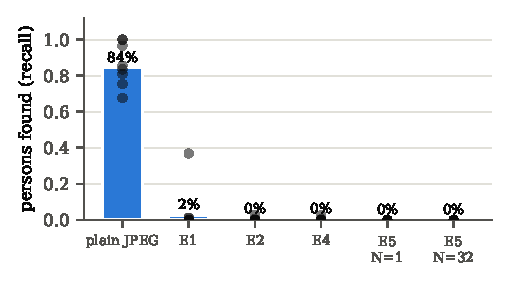
\includegraphics[width=\columnwidth]{figures/fig_recognition.pdf}
\caption{Share of the persons that a Faster R-CNN detector finds in the original frames and also finds, at the same place, in the eavesdropper's pictures (bars: pooled over \RecSources{} sources; dots: per source).}
\label{fig:recognition}
\end{figure}
% generated by paper/make_assets.py from paper/data -- do not edit
\begin{table}[t]
\caption{Person detection (Faster R-CNN, COCO) in the eavesdropper's pictures: recall (\%) of the persons found in the original frame, a detection in any attacker picture counting when it overlaps the original box (IoU $\ge$ 0.3). Sources with at least one person; 40 frames each (Kodak: 24 images).}
\label{tab:recognition}
\centering\small\setlength{\tabcolsep}{3pt}
\resizebox{\columnwidth}{!}{%
\begin{tabular}{lrrrrrrr}
\toprule
Source & Persons & Plain & E1 & E2 & E4 & E5/1 & E5/32 \\
\midrule
Trailer A & 69 & 75 & 0 & 0 & 0 & 0 & 0 \\
Trailer B & 63 & 81 & 0 & 0 & 0 & 0 & 0 \\
Talk A & 248 & 85 & 1 & 0 & 0 & 0 & 0 \\
Talk B & 38 & 100 & 37 & 3 & 3 & 0 & 0 \\
Phone A & 388 & 84 & 1 & 0 & 0 & 0 & 0 \\
Sintel & 34 & 68 & 0 & 0 & 0 & 0 & 0 \\
Tears of Steel & 29 & 97 & 0 & 0 & 0 & 0 & 0 \\
Kodak & 31 & 100 & 0 & 0 & 0 & 0 & 0 \\
\bottomrule
\end{tabular}}
\end{table}

Correlations measure whether a picture is in the right place; a person looking at the screen needs no such alignment. We therefore ran an off-the-shelf person detector, Faster R-CNN~\cite{ren2015} with a ResNet-50 FPN backbone trained on COCO, on the original and on every picture an eavesdropper can make, at a score threshold of 0.5, and counted an original person as found if an attacker picture has a detection overlapping it by an IoU of at least 0.3. Fig.~\ref{fig:recognition} and Table~\ref{tab:recognition} show the result over \RecPersons{} persons. On unprotected frames the detector finds \RecPlainMin--\RecPlainMax\,\% of them. Sign-only encryption already defeats it on most sources (\RecEonePooled\,\% pooled), but not on one talking-head clip (\RecEoneMax\,\%); under E2 and E4 it finds at most \RecEtwoFourMax\,\% on any source, and under E5 none. Detections anywhere in a frame, regardless of position, occur in at most \RecHitEtwoFiveMax\,\% of the frames with a person under E2--E5, about as often as false alarms on frames without one.

\subsection{Restart interval}\label{sec:restart}
% generated by paper/make_assets.py from paper/data -- do not edit
\begin{table}[t]
\caption{E5 with $N$ macroblocks per restart segment, mean over 8 sources. Overhead vs.\ E4 without markers; NZCA correlation; Succ.: segments chained to their true successor by a beam-search solver (chance).}
\label{tab:restart}
\centering\small\setlength{\tabcolsep}{3.5pt}
\resizebox{\columnwidth}{!}{%
\begin{tabular}{lccccc}
\toprule
$N$ & Segments & Perm.\ bits & Overhead (\%) & NZCA & Succ.\ (chance) \\
\midrule
E4 (no shuffle) & -- & -- & -- & 0.81 & -- \\
1 & 300 & 2041 & 14.2 & 0.00 & 0.02 (0.00) \\
4 & 75 & 363 & 3.5 & 0.01 & 0.03 (0.01) \\
8 & 38 & 149 & 1.8 & 0.03 & 0.03 (0.03) \\
10 & 30 & 108 & 1.4 & 0.02 & 0.08 (0.03) \\
32 & 10 & 22 & 0.5 & 0.03 & 0.25 (0.11) \\
\bottomrule
\end{tabular}}
\end{table}

E5 as specified costs \RiOverheadOneMin--\RiOverheadOneMax\,\% over the same E4 coefficients at 320$\times$240, as~\eqref{eq:e5cost} predicts: a two-byte marker per macroblock, padding and restarted DC prediction. $N$ macroblocks per segment reduce this to \RiOverheadFour\,\% at $N{=}4$ and \RiOverheadThirtyTwo\,\% at $N{=}32$ (Table~\ref{tab:restart}). Hirose et al.\ found that the non-zero counting attack reveals the scene unless the restart segments are permuted, and partly again when the restart interval is large~\cite{hirose2024}. Without the shuffle, our NZCA map correlates \RiNzcaEfourMin--\RiNzcaEfourMax{} with the original's block edge energy; with it, at most \RiNzcaEfiveMax{} for every $N$ we tried. At $N{=}32$, however, only \RiSegThirtyTwo{} segments remain, each an intact strip of 32 macroblocks, and a beam-search solver that chains segments by border continuity links \RiSuccThirtyTwoMin--\RiSuccThirtyTwoMax{} of them to their true successor on the real clips (chance \RiChanceThirtyTwo), against at most \RiSuccSmallMax{} for $N\le 8$. We keep $N{=}1$ and do not claim that longer intervals are safe.

\subsection{Standard metrics and key sensitivity}
% generated by paper/make_assets.py from paper/data -- do not edit
\begin{table}[t]
\caption{Standard image-encryption metrics, mean over 8 sources (5--6 frames each). Wrong key: the receiver's output with a key that differs in one bit, compared with the original (SSIM) and with the right decryption (NPCR/UACI, \%). 1-pixel: NPCR between two ciphertexts of frames that differ in one pixel, same key and nonce. Ideal values for a full-image cipher: NPCR 99.6, UACI 33.5, entropy 8, adjacent correlation 0.}
\label{tab:std}
\centering\small\setlength{\tabcolsep}{3pt}
\resizebox{\columnwidth}{!}{%
\begin{tabular}{lccccc}
\toprule
Level & Wrong-key SSIM & NPCR / UACI & 1-pixel NPCR & Entropy & Adj.\ corr. \\
\midrule
plain & -- & -- & -- & 5.88 & 0.93 \\
E1 & 0.58 & 70.3 / 4.9 & 33.8 & 6.02 & 0.89 \\
E2 & 0.27 & 89.8 / 46.3 & 35.5 & 5.40 & 0.92 \\
E3 & 0.25 & 87.8 / 42.9 & 33.3 & 5.25 & 0.91 \\
E4 & 0.24 & 88.8 / 47.5 & 34.5 & 5.14 & 0.91 \\
E5 & 0.13 & 95.8 / 35.8 & 46.8 & 7.07 & 0.88 \\
\bottomrule
\end{tabular}}
\end{table}

On all \StdSources{} sources (Table~\ref{tab:std}), key sensitivity holds: a one-bit key change makes E5 decryption differ in \StdNpcrEfiveMin--\StdNpcrEfiveMax\,\% of the pixels (SSIM $\le$\StdWrongSsimEfiveMax); in practice the receiver rejects such a frame because its tag fails. The other metrics assume a cipher that turns the image into noise: the 8$\times$8 block structure survives, so adjacent-pixel correlation stays at \StdCorrMin--\StdCorrMax{} and entropy rises only under E5 (\StdEntropyPlain{} to \StdEntropyEfive{} bits), and the 1-pixel NPCR (at most \StdPixelNpcrMax\,\%) measures diffusion, which a stream cipher with a fresh nonce per frame does not need: a one-pixel change of the plaintext under the same nonce never happens, because every frame has its own counter.

\subsection{Security summary}
Against goal G1, E1 is broken by a trained network and E2--E4 leak the outline under every attack we tried, however many bits they encrypt; E5 removed the outline under all of them, including known plaintext, chosen plaintext, two puzzle solvers, sign recovery and two trained networks, at a byte cost of \RiOverheadOneMin--\RiOverheadOneMax\,\%. What E5 leaks is the frame's colour statistics and its size; Section~\ref{sec:discussion} treats the latter.
